%% Minimal KTH thesis for:
%% "Parallel Programming with Off-Heap Memory in Scala Native"
%%
%% Based on the KTH thesis template (kththesis.cls).
%% Compile with: xelatex/lualatex + bibtex  (Overleaf default: XeLaTeX)

% Make it possible to conditionally depend on the TeX engine used
\RequirePackage{ifxetex}
\RequirePackage{ifluatex}
\newif\ifxeorlua
\ifxetex\xeorluatrue\fi
\ifluatex\xeorluatrue\fi

\ifxeorlua
  \RequirePackage{expl3}
  \RequirePackage{etoolbox}   %% needed before \documentclass (kththesis.cls uses \newtoggle at line 5)
  \ExplSyntaxOn
  \ExplSyntaxOff
\else
  \RequirePackage{expl3}
  \ExplSyntaxOn
  \pdf_version_gset:n{1.5}
  \ExplSyntaxOff
\fi

%% Commands to disable/re-enable packages (requires etoolbox)
\makeatletter
\newcommand{\disablepackage}[2]{\disable@package@load{#1}{#2}}
\newcommand{\reenablepackage}[1]{\reenable@package@load{#1}}
\makeatother
\ifxeorlua
  \disablepackage{transparent}{}
\fi

\documentclass[
  english,   % thesis language
  bibtex,    % bibliography processor
]{kththesis}

% Bibliography style (bibtex path; must be in preamble)
\iftoggle{biblatex}{
  \usepackage[style=ieee,citestyle=numeric-comp]{biblatex}
  \addbibresource{thesis_references.bib}
}{
  \bibliographystyle{bibstyle/myIEEEtran}
}

% Core packages
\input{lib/includes}
\input{lib/kthcolors}
\input{lib/defines}

% Hyperref — no engine-specific options; let the driver auto-detect
\iftoggle{biblatex}{
  \usepackage[plainpages=false]{hyperref}
}{
  \usepackage[
    backref=page,
    pagebackref=false,
    plainpages=false,
    unicode=true,
    bookmarks=true,
    bookmarksopen=false,
    pdfpagemode=UseNone,
    destlabel,
    pdfencoding=auto,
  ]{hyperref}
}
\usepackage[all]{hypcap}

% Glossaries (must come after hyperref)
\usepackage[acronym, style=super, section=section, nonumberlist, nomain, nopostdot]{glossaries}
\setlength{\glsdescwidth}{0.75\textwidth}
\usepackage[]{glossaries-extra}
\input{lib/includes-after-hyperref}
\makeglossaries

% Acronyms
\ifxeorlua
  \input{lib/acronyms}
\else
  \input{lib/acronyms-for-pdflatex}
\fi
\ifglsentryexists{GC}{}{\newacronym{GC}{GC}{garbage collection}}
\ifglsentryexists{JVM}{}{\newacronym{JVM}{JVM}{Java Virtual Machine}}
\ifglsentryexists{LLVM}{}{\newacronym{LLVM}{LLVM}{Low Level Virtual Machine}}
\ifglsentryexists{DEBS}{}{%
  \newacronym{DEBS}{DEBS}{Distributed and Event-Based Systems}%
}
\input{lib/placeHolder_lbx_files}

% Configuration (author, supervisor, degree details, …)
%% Configuration for: Parallel Programming with Off-Heap Memory in Scala Native

\date{\today}

\title{Parallel Programming with Off-Heap Memory in Scala Native}
\subtitle{}

\alttitle{Parallell programmering med off-heap-minne i Scala Native}
\altsubtitle{}

% --- Degree details (MSc thesis, EECS) ---
\courseCycle{2}
\courseCode{DA231X}
\courseCredits{30.0}
\programcode{TCSCM}
\degreeName{Master's Programme, Computer Science, 120 credits}
\subjectArea{Computer Science}

% --- Author Information ---
\authorsLastname{Lastname}
\authorsFirstname{Firstname}
\email{XXXXXXXXXXXX@kth.se}
\kthid{u1XXXXXX}
\authorsSchool{\schoolAcronym{EECS}}
\authorCityCountryDate{\MONTH\enspace\the\year}

% --- Supervisor Information ---
\supervisorAsLastname{Haller}
\supervisorAsFirstname{Philipp}
\supervisorAsEmail{phaller@kth.se}
\supervisorAsKTHID{u1XXXXXX}
\supervisorAsSchool{\schoolAcronym{EECS}}
\supervisorAsDepartment{Computer Science}

% --- Examiner Information ---
\examinersLastname{ExaminersLastname}
\examinersFirstname{ExaminersFirstname}
\examinersEmail{XXXXXXXXXXXX@kth.se}
\examinersKTHID{u1XXXXXX}
\examinersSchool{\schoolAcronym{EECS}}
\examinersDepartment{Computer Science}

% --- National Subject Categories ---
% 10201 = Computer Science
\nationalsubjectcategories{10201}

% --- UN Sustainable Development Goals ---
% SDG 9: Industry, Innovation and Infrastructure
\SDGs{9}


% Keywords stored for PDF metadata and abstract pages
\EnglishKeywords{Scala Native, off-heap memory, parallel collections, garbage collection, performance, stream processing, benchmarking}
\SwedishKeywords{Scala Native, off-heap-minne, parallella samlingar, skräpinsamling, prestanda, strömbearbetning, benchmarking}

% PDF metadata
\input{lib/pdf_related_includes}

\hypersetup{colorlinks=true, urlcolor=blue, linkcolor=black, citecolor=black}

% -----------------------------------------------------------------------
\begin{document}
\selectlanguage{english}

\pagenumbering{alph}
\kthcover
\clearpage\thispagestyle{empty}\mbox{}
\titlepage
\bookinfopage

% ========================  FRONT MATTER  ================================
\frontmatter
\setcounter{page}{1}

% ---- English abstract --------------------------------------------------
\begin{abstract}
  \markboth{\abstractname}{}
\begin{scontents}[store-env=lang]
eng
\end{scontents}
\begin{scontents}[store-env=abstracts,print-env=true]

The Scala programming language offers excellent support for concurrent and
distributed programming through abstractions such as futures and actors.
Standard Scala relies on garbage collection (GC) for automatic memory
management; however, GC introduces efficiency losses and increased latency
that are unacceptable in performance-critical systems.

This thesis explores the use of \textit{off-heap memory} for parallel programs
compiled with the Scala Native compiler, with the goal of avoiding GC overhead
entirely.  The central hypothesis is that parallel programs that process
significant amounts of data---for example, stream-processing pipelines---can
benefit substantially from the higher efficiency of off-heap memory zones
already supported by Scala Native.

The project designs and implements a library for parallel collections (with an
\gls{API} similar to the standard Scala parallel-collections library) whose
memory is allocated in off-heap zones.  A suite of representative benchmark
programs and a curated selection of real-world datasets (drawn from the
\gls{DEBS} Grand Challenges) are used to evaluate performance relative to
on-heap parallel collections.

The expected contributions are: (i) a reusable open-source library for
off-heap parallel collections in Scala Native; (ii) a benchmark harness for
evaluating off-heap vs.\ on-heap performance; and (iii) empirical insights
that will inform a research paper on the safety of off-heap memory zones via
types, to be completed in collaboration with a PhD student.

\end{scontents}

\subsection*{Keywords}
\begin{scontents}[store-env=keywords,print-env=true]
\InsertKeywords{english}
\end{scontents}
\end{abstract}

\cleardoublepage

% ---- Swedish abstract --------------------------------------------------
\babelpolyLangStart{swedish}
\begin{abstract}
  \markboth{\abstractname}{}
\begin{scontents}[store-env=lang]
swe
\end{scontents}
\begin{scontents}[store-env=abstracts,print-env=true]

Programmeringsspråket Scala erbjuder utmärkt stöd för concurrent och
distribuerad programmering via abstraktioner som futures och aktörer.
Standard-Scala förlitar sig på skräpinsamling (GC) för automatisk
minneshantering, men GC medför effektivitetsförluster och ökad latens som
är oacceptabla i prestandakritiska system.

Den här avhandlingen undersöker användningen av \textit{off-heap-minne} för
parallella program kompilerade med Scala Native-kompilatorn, i syfte att
helt undvika GC-overhead.  Projektet utformar och implementerar ett bibliotek
för parallella samlingar vars minne allokeras i off-heap-zoner, utvärderar
prestanda med hjälp av riktmärkesprogram och verkliga datamängder, och
bidrar med empiriska insikter till en kommande forskningsartikel om
typsäkerhet för off-heap-minneszoner.

\end{scontents}

\subsection*{Nyckelord}
\begin{scontents}[store-env=keywords,print-env=true]
\InsertKeywords{swedish}
\end{scontents}
\end{abstract}
\cleardoublepage
\babelpolyLangStop{swedish}

% ---- Acknowledgements --------------------------------------------------
\section*{Acknowledgments}
\markboth{Acknowledgments}{}

I would like to thank Philipp Haller for the inspiring thesis proposal,
valuable guidance, and the opportunity to contribute to ongoing research on
safe off-heap memory in Scala Native.

\acknowlegmentssignature

% ---- Tables of contents / figures / tables -----------------------------
\fancypagestyle{plain}{}
\renewcommand{\chaptermark}[1]{\markboth{#1}{}}
\tableofcontents
  \markboth{\contentsname}{}

\cleardoublepage
\listoffigures
\cleardoublepage
\listoftables
\cleardoublepage

% Glossary / acronyms
\newglossarystyle{mylong}{%
  \setglossarystyle{long}%
  \renewenvironment{theglossary}{\begin{longtable}{lp{\glsdescwidth}}}{\end{longtable}}%
}
\printglossary[style=mylong, type=\acronymtype, title={List of acronyms and abbreviations}]

\label{pg:lastPageofPreface}

% ========================  MAIN MATTER  =================================
\mainmatter
\glsresetall
\renewcommand{\chaptermark}[1]{\markboth{#1}{}}
\selectlanguage{english}

% ------------------------------------------------------------------------
\chapter{Introduction}
\label{ch:introduction}

This chapter describes the problem addressed by this thesis, its context,
the goals of the project, and the structure of the document.

\section{Background}
\label{sec:background}

The Scala programming language is known for its excellent support for
concurrent and distributed programming through abstractions such as futures
and actors~\cite{haller_scala_actors}.  Standard Scala programs rely on
garbage collection (\gls{GC}) for automatic memory management.  While GC
simplifies programming, it introduces unpredictable pauses and efficiency
losses that are unacceptable in performance-critical, data-intensive
systems~\cite{gog_broom_2015}.

Scala Native~\cite{scala_native} is an ahead-of-time compiler and runtime
for Scala that already provides support for \textit{off-heap memory zones}:
manually managed memory regions that bypass the \gls{GC} entirely.  However,
no parallel-collections library that exploits off-heap zones currently exists
for Scala Native.

\section{Problem Statement}
\label{sec:problem}

Can off-heap parallel collections in Scala Native deliver measurably better
throughput and lower latency than their on-heap counterparts for
data-intensive stream-processing workloads?

\section{Purpose}
\label{sec:purpose}

The purpose of this project is to advance the state of the art in
high-performance parallel programming for Scala Native, providing both
practitioners (who need predictable, low-latency data processing) and
researchers (who study the safety of off-heap memory) with concrete tools
and empirical evidence.

\section{Goals}
\label{sec:goals}

The project is divided into three concrete sub-goals:

\begin{enumerate}
  \item \textbf{Library design and implementation.}  Design and implement a
        library for parallel collections---with an \gls{API} similar to the
        standard Scala parallel-collections library~\cite{prokopec_parallel_2011}---whose
        memory is allocated in off-heap zones supported by Scala Native.

  \item \textbf{Benchmarking suite.}  Design and implement a suite of
        representative benchmark programs that evaluate the performance of
        off-heap parallel collections against on-heap parallel collections.

  \item \textbf{Dataset curation and experimental evaluation.}  Gather and
        curate a selection of datasets (drawing on the \gls{DEBS} Grand
        Challenges~\cite{debs_grand_challenges}) and carry out a systematic
        experimental evaluation.
\end{enumerate}

\section{Research Methodology}
\label{sec:methodology}

The project follows a design-science methodology: an artefact (the library)
is constructed, benchmarked against controlled baselines, and the results
are analysed to answer the research question.  Performance measurements
will be collected using established \gls{JVM}/native micro-benchmarking
practices to minimise noise.

\section{Delimitations}
\label{sec:delimitations}

This thesis focuses exclusively on the Scala Native runtime; \gls{JVM}-based
Scala is out of scope.  Type-system guarantees for memory safety are studied
in a parallel research effort and are therefore not a deliverable of this
thesis.

\section{Structure of the Thesis}
\label{sec:structure}

Chapter~\ref{ch:background} presents background material on off-heap memory,
Scala Native, and parallel collections.
Chapter~\ref{ch:methods} describes the research and engineering methodology.
Chapter~\ref{ch:design} presents the library design and implementation.
Chapter~\ref{ch:evaluation} presents the experimental evaluation.
Chapter~\ref{ch:conclusions} draws conclusions and outlines future work.

% ------------------------------------------------------------------------
\chapter{Background and Related Work}
\label{ch:background}

\section{Garbage Collection and Its Costs}

Garbage collection automates memory reclamation but at the cost of stop-the-world
pauses and unpredictable throughput degradation.  Gog \etal~\cite{gog_broom_2015}
demonstrated that eliminating GC from big-data systems can yield substantial
performance improvements.

\section{Scala Native and Off-Heap Zones}

Scala Native~\cite{scala_native} exposes \texttt{Zone}-based off-heap allocation: a semi-automatic memory management
technique that binds allocations to a temporary scope in the program~\cite{scala_native_interop}. Zones
automatically clean up memory as soon as execution exits the zone, making them the
preferred way to allocate temporary unmanaged memory without invoking the garbage
collector. Memory is obtained from the operating system, bypassing the \gls{GC} entirely,
and is freed deterministically when the zone exits scope. Within a zone, the \texttt{alloc}
function requests memory sufficient to contain a specified number of values of a given
type, with memory zeroed out by default. As shown in the thesis project, zones enable
high-performance parallel collection implementations where off-heap data structures can
avoid heap allocation entirely, provided memory captures are carefully scoped to the zone
lifetime.

\section{Parallel Collections}

The standard Scala parallel-collections library~\cite{prokopec_parallel_2011}
provides high-level data-parallel abstractions (e.g., \texttt{par.map},
\texttt{par.filter}) over \gls{JVM} heap memory.  Prokopec \etal describe the
generic framework underlying these collections.

\section{DEBS Grand Challenges}

The \gls{DEBS} Grand Challenges~\cite{debs_grand_challenges} supply realistic,
publicly available datasets for event-driven stream-processing benchmarks,
making them a natural choice for evaluating throughput and latency.

\section{Summary}

Table~\ref{tab:related_work_summary} summarises the key related works and
their relevance to this thesis.

\begin{table}[!ht]
  \centering
  \caption{Summary of related work}
  \label{tab:related_work_summary}
  \begin{tabular}{lll}
    \hline
    \textbf{Work} & \textbf{Topic} & \textbf{Relevance} \\
    \hline
    Gog \etal~\cite{gog_broom_2015}           & GC elimination in big-data & Motivation \\
    Scala Native~\cite{scala_native}           & Native Scala runtime       & Platform   \\
    Prokopec \etal~\cite{prokopec_parallel_2011} & Parallel collections     & API design \\
    DEBS~\cite{debs_grand_challenges}          & Benchmark datasets         & Evaluation \\
    \hline
  \end{tabular}
\end{table}

% ------------------------------------------------------------------------
\chapter{Method}
\label{ch:methods}

This chapter describes the engineering and research methodology used to
achieve the project goals stated in Section~\ref{sec:goals}.

\section{Research Process}
\label{sec:researchProcess}

The project follows iterative design-science cycles: design, implement,
measure, and refine.

\section{Library Design Methodology}

The library \gls{API} will be modelled closely on the existing Scala
parallel-collections \gls{API}~\cite{prokopec_parallel_2011} to minimise the
learning curve for Scala developers.  Off-heap allocation will be provided
via Scala Native zones.  Thread parallelism will be achieved using
platform threads coordinated through a fixed-size thread pool.

\section{Benchmarking Methodology}
\label{sec:benchmarkingMethod}

Benchmarks will measure wall-clock throughput (events/s) and end-to-end
latency (ms) for representative stream-processing pipelines.  Each benchmark
will be repeated sufficiently many times to obtain stable estimates;
warm-up phases will be excluded from reported measurements.

\section{Experimental Design}
\label{sec:experimentalDesign}

\begin{itemize}
  \item \textbf{Independent variable:} memory allocation strategy
        (off-heap zone vs.\ on-heap \gls{GC}).
  \item \textbf{Dependent variables:} throughput, latency, peak memory usage.
  \item \textbf{Datasets:} curated subset of \gls{DEBS} Grand Challenge data.
  \item \textbf{Hardware:} a single multi-core machine with fixed clock speed
        to minimise variability.
\end{itemize}

% ------------------------------------------------------------------------
\chapter{Library Design and Implementation}
\label{ch:design}

\section{Architecture Overview}

% TODO: describe library architecture

\section{Off-Heap Parallel Collections API}

% TODO: describe public API

\section{Implementation}

% TODO: describe implementation details

% ------------------------------------------------------------------------
\chapter{Experimental Evaluation}
\label{ch:evaluation}

\section{Experimental Setup}
Experiments were executed from the project root at
`/Users/a.mordovskiy/scala_1105` on the author's macOS development machine.
The benchmark binary was built with `sbt nativeLink` (see
`build.sbt` in the project root). Profiling was performed using the
`samply` sampler following the Scala Native profiling guide
(https://scala-native.org/en/stable/user/profiling.html). In brief:

\begin{itemize}
  \item build the native binary: `sbt clean nativeLink`
  \item run the benchmark binary (or start it via sbt)
  \item run `samply` to collect samples while the benchmark executes and
        export a flamegraph according to the `samply` instructions
\end{itemize}

The flamegraphs in Figures~\ref{fig:profiler_structs} and
\ref{fig:profiler_optimized} were generated with this workflow.

\section{Key Findings: Struct Tagging Overhead}
\label{sec:structTagging}

During initial profiling of off-heap parallel collections with \texttt{CStruct}-based
node representations, we observed significant \gls{GC} activity despite allocating
primary data structures in zones (off-heap).  Profiling revealed that over 50\% of
runtime was spent in calls to \texttt{scalanative\_GC\_alloc\_small} and
\texttt{Tag\$CStruct1\$.apply}, even when the heap-allocated payload was negligible.

The root cause is the implicit materialization of \texttt{Tag} instances for
\texttt{CStruct} types during zone allocation operations.  Each access to a struct
field in a tight loop can trigger tag instantiation on the heap, negating
off-heap allocation benefits.  Explicit tag materialization via
\texttt{Tag.materializeCStruct1Tag[T]} only partially mitigates this overhead.

This finding suggests that efficient off-heap parallel collections in Scala Native
should prefer alternative representations (e.g., flat, untagged arrays or
primitive-backed data structures) when possible, or employ specialized API designs
that front-load tag instantiation outside performance-critical loops.
These insights inform the library design choices discussed in Chapter~\ref{ch:design}.

\begin{figure}[!ht]
  \centering
  \begin{minipage}{0.48\textwidth}
    \centering
    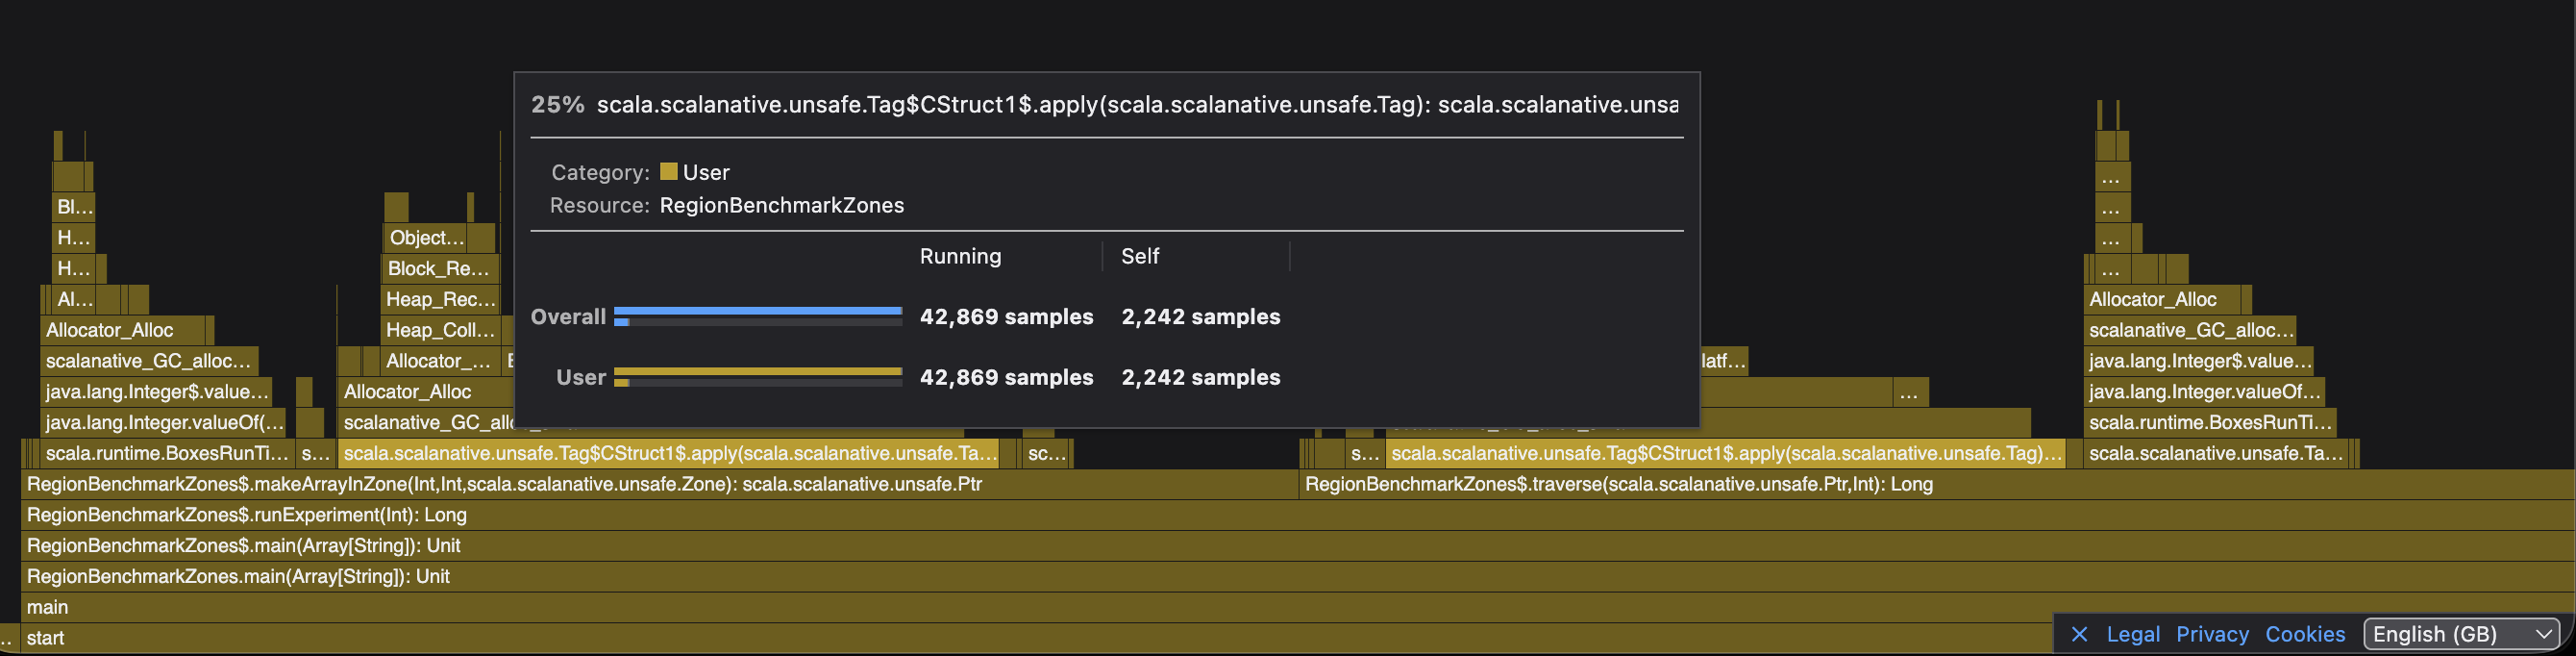
\includegraphics[width=\textwidth]{figures/profiler_structs_overhead.png}
    \caption{Profiler output with \texttt{CStruct}-based nodes: 25\% of runtime
    spent in \texttt{Tag\$CStruct1\$.apply} heap allocations.}
    \label{fig:profiler_structs}
  \end{minipage}
  \hfill
  \begin{minipage}{0.48\textwidth}
    \centering
    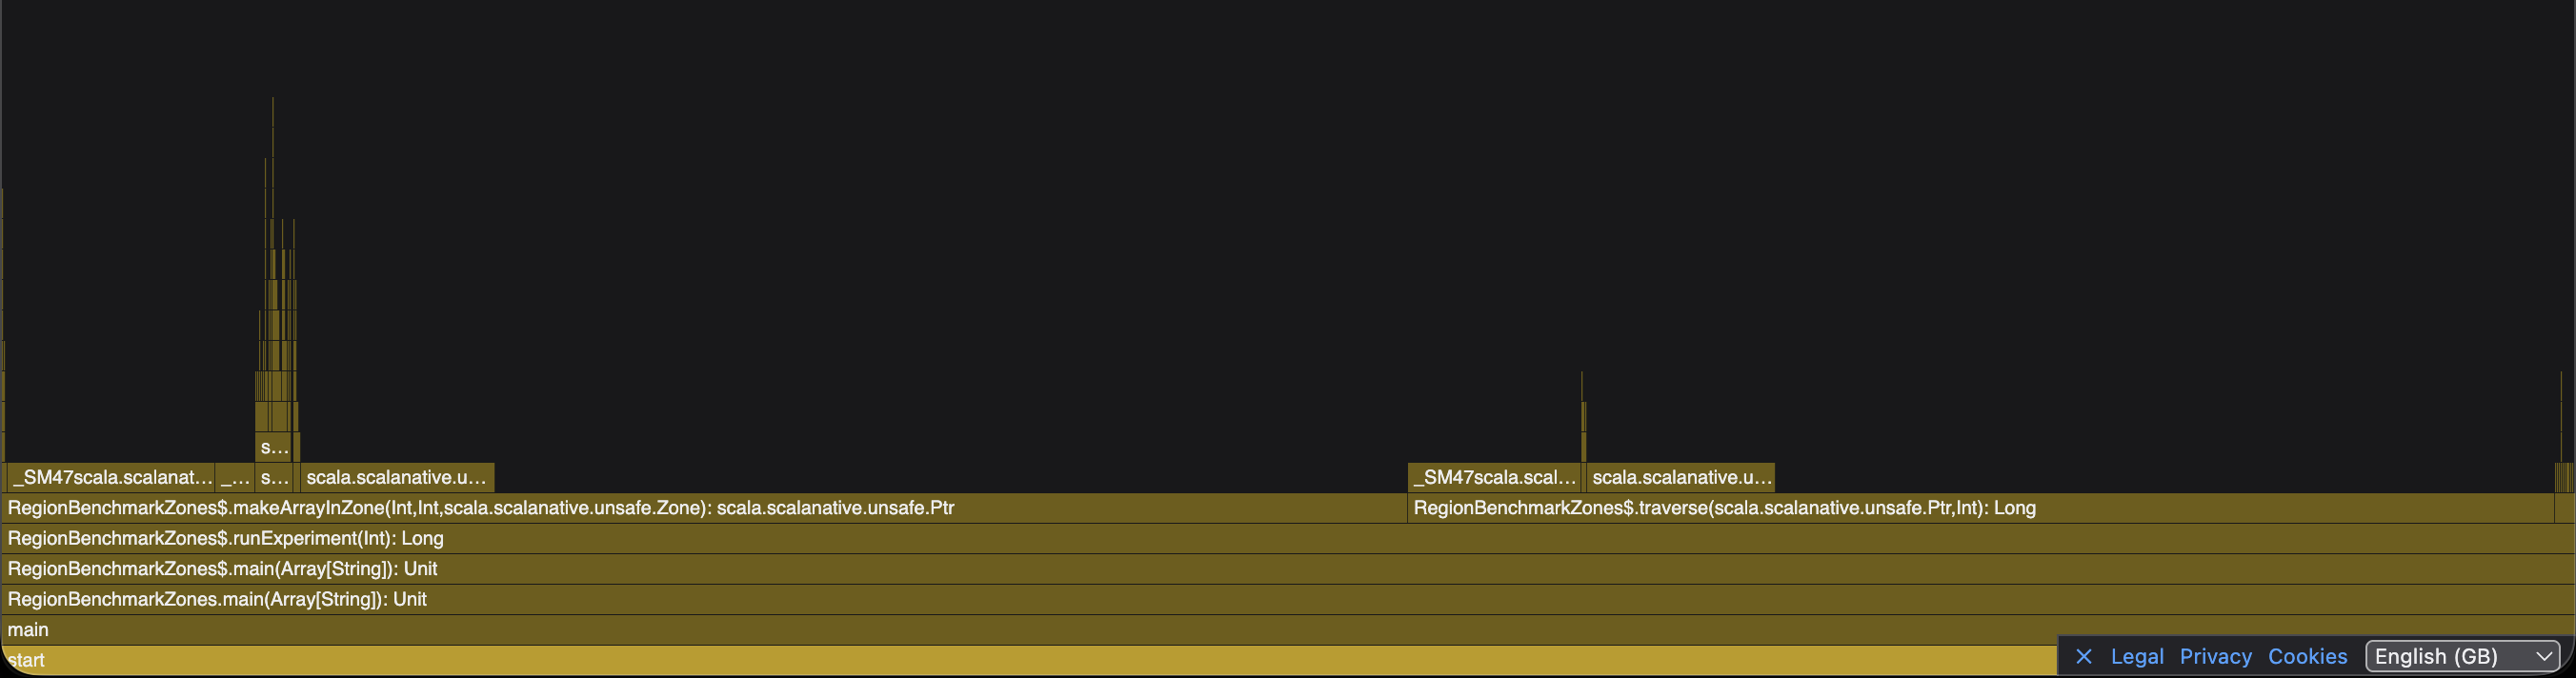
\includegraphics[width=\textwidth]{figures/profiler_baseline_optimized.png}
    \caption{Profiler output with optimized representation (primitive-backed arrays):
    negligible heap allocation overhead.}
    \label{fig:profiler_optimized}
  \end{minipage}
\end{figure}

Figure~\ref{fig:profiler_structs} and Figure~\ref{fig:profiler_optimized} contrast profiler
outputs from two implementations. The struct-based version exhibits significant heap
churn from implicit tag instantiation, while the optimized baseline achieves
near-zero allocation overhead. This comparison provides empirical motivation for
preferring flat data layouts in performance-critical allocation-free code paths.

\section{Results}

% TODO: tables and figures with benchmark results

\section{Discussion}

% TODO: interpret results, answer research question

% ------------------------------------------------------------------------
\chapter{Conclusions}
\label{ch:conclusions}

\section{Summary of Contributions}

% TODO: summarise what was built and found

\section{Future Work}
\label{sec:future_work}

\begin{itemize}
  \item Integration of type-system guarantees for off-heap memory safety
        (ongoing parallel research with a PhD student).
  \item Extension of the library to distributed settings.
  \item Presentation of results at a leading Scala conference.
\end{itemize}

% ========================  BACK MATTER  =================================
\iftoggle{biblatex}{
  \printbibliography
}{
  \bibliography{thesis_references}
}

\end{document}
